% Previous horizontal figure preserved for review:
% % Native TikZ source for the design-alternative loading-time figure.
% % Values are the single-run measurements promoted in:
% %   vcomp/experiments/results/paper_figure4_loading_time_1tb_single.tsv
% % Dataset: 1,000 GiB logical input; key/value sizes: 24 B / 1,000 B.
% % The natural width is close to one USENIX column so that surrounding
% % \resizebox{\columnwidth}{!}{...} introduces little font scaling.
% \begingroup
% \definecolor{altBaseline}{HTML}{5B5B5B}
% \definecolor{altAdoc}{HTML}{8E5AA9}
% \definecolor{altBlobdb}{HTML}{D55E00}
% \definecolor{altFlush}{HTML}{E69F00}
% \definecolor{altLast}{HTML}{F0A83B}
% \definecolor{altFillseq}{HTML}{009E73}
% \definecolor{altFillseqOw}{HTML}{4AAE91}
% \definecolor{altFtwo}{HTML}{0072B2}
% \begin{tikzpicture}[
%     x=1cm,
%     y=1cm,
%     font=\small,
%     axis/.style={draw=black!80, line width=0.50pt},
%     grid/.style={draw=black!16, line width=0.40pt},
%     baselinebar/.style={draw=black!80, fill=altBaseline, line width=0.45pt},
%     adocbar/.style={draw=black!80, fill=altAdoc, line width=0.45pt},
%     blobdbbar/.style={draw=black!80, fill=altBlobdb, line width=0.45pt},
%     flushbar/.style={draw=black!80, fill=altFlush, line width=0.45pt},
%     lastbar/.style={draw=black!80, fill=altLast, line width=0.45pt},
%     fillseqbar/.style={draw=black!80, fill=altFillseq, line width=0.45pt},
%     fillseqowbar/.style={draw=black!80, fill=altFillseqOw, line width=0.45pt},
%     f2loadbar/.style={draw=black!80, fill=altFtwo, line width=0.45pt}
% ]
% \path[use as bounding box] (-0.03,-0.34) rectangle (8.22,5.25);
% 
% % Linear x scale: 0--90 minutes over 5.10 cm.
% \foreach \value/\x in {0/2.15,30/3.85,60/5.55,90/7.25} {
%     \draw[grid] (\x,0.48) -- (\x,5.15);
%     \draw[axis] (\x,0.42) -- (\x,0.48);
%     \node[anchor=north, font=\scriptsize] at (\x,0.37) {\value};
% }
% \draw[axis] (2.15,0.48) -- (7.48,0.48);
% \draw[axis] (2.15,0.48) -- (2.15,5.15);
% 
% % y / method / measured minutes / displayed value / bar style
% % Exact promoted values are retained for bar geometry; labels round to one
% % decimal place, matching the precision used by the paper text.
% \foreach \y/\method/\minutes/\shown/\barstyle in {
%     4.86/{Baseline}/55.3333/55.3/baselinebar,
%     4.28/{ADOC}/68.7000/68.7/adocbar,
%     3.70/{BlobDB}/28.5333/28.5/blobdbbar,
%     3.12/{Flush-only}/16.2167/16.2/flushbar,
%     2.54/{Last-comp}/83.7667/83.8/lastbar,
%     1.96/{Fillseq}/20.9500/21.0/fillseqbar,
%     1.38/{Fillseq+OW}/29.0833/29.1/fillseqowbar,
%     0.80/{F2Load}/1.7000/1.7/f2loadbar%
% } {
%     \pgfmathsetmacro{\barend}{2.15 + 0.0566666667*\minutes}
%     \draw[\barstyle] (2.15,\y-0.20) rectangle (\barend,\y+0.20);
%     \node[anchor=east, font=\scriptsize] at (2.02,\y) {\method};
%     \node[anchor=west, font=\scriptsize] at (\barend+0.10,\y) {\shown};
% }
% 
% \node[anchor=north, font=\small] at (4.82,-0.04) {Loading time (min)};
% \end{tikzpicture}
% \endgroup

% Previous plotted version preserved for review:
% % Loading: vcomp/experiments/results/paper_figure4_loading_time_1tb_single.tsv
% % Reads: vcomp/experiments/results/paper_figure4_uniform_read_cache_5m_single.tsv
% % One run per cell; all measured values are unchanged by this layout revision.
% \begingroup
% \definecolor{vb0}{HTML}{5B5B5B}
% \definecolor{vb1}{HTML}{8E5AA9}
% \definecolor{vb2}{HTML}{D55E00}
% \definecolor{vb3}{HTML}{E69F00}
% \definecolor{vb4}{HTML}{F0A83B}
% \definecolor{vb5}{HTML}{009E73}
% \definecolor{vb6}{HTML}{4AAE91}
% \definecolor{vb7}{HTML}{0072B2}
% \begin{tikzpicture}[x=1cm,y=1cm,font=\small,
% axis/.style={draw=black!80,line width=0.5pt},
% grid/.style={draw=black!16,line width=0.4pt}]
% \path[use as bounding box] (0,0) rectangle (8.500,5.150);
% \draw[grid] (0.85,1.4000) -- (8.3500,1.4000);
% \draw[axis] (0.79,1.4000) -- (0.85,1.4000);
% \node[font=\fontsize{7}{8}\selectfont,anchor=east] at (0.7300,1.4000) {0};
% \draw[grid] (0.85,2.5000) -- (8.3500,2.5000);
% \draw[axis] (0.79,2.5000) -- (0.85,2.5000);
% \node[font=\fontsize{7}{8}\selectfont,anchor=east] at (0.7300,2.5000) {30};
% \draw[grid] (0.85,3.6000) -- (8.3500,3.6000);
% \draw[axis] (0.79,3.6000) -- (0.85,3.6000);
% \node[font=\fontsize{7}{8}\selectfont,anchor=east] at (0.7300,3.6000) {60};
% \draw[grid] (0.85,4.7000) -- (8.3500,4.7000);
% \draw[axis] (0.79,4.7000) -- (0.85,4.7000);
% \node[font=\fontsize{7}{8}\selectfont,anchor=east] at (0.7300,4.7000) {90};
% \draw[axis] (0.85,1.4000) -- (8.3500,1.4000);
% \draw[axis] (0.85,1.4000) -- (0.85,4.7000);
% \node[font=\fontsize{7}{8}\selectfont,rotate=90,anchor=south] at (0.1000,3.0500) {Loading time (min)};
% % baseline: 55.33330000 min
% \draw[draw=black!80,line width=0.4pt,fill=vb0] (1.03000,1.40000) rectangle (1.63000,3.42889);
% \node[font=\fontsize{7}{8}\selectfont,anchor=south] at (1.3300,3.5089) {55.3};
% \node[font=\fontsize{7}{8}\selectfont,rotate=45,anchor=north east] at (1.3300,1.3000) {Baseline};
% % adoc: 68.70000000 min
% \draw[draw=black!80,line width=0.4pt,fill=vb1] (1.96000,1.40000) rectangle (2.56000,3.91900);
% \node[font=\fontsize{7}{8}\selectfont,anchor=south] at (2.2600,3.9990) {68.7};
% \node[font=\fontsize{7}{8}\selectfont,rotate=45,anchor=north east] at (2.2600,1.3000) {ADOC};
% % blobdb: 28.53330000 min
% \draw[draw=black!80,line width=0.4pt,fill=vb2] (2.89000,1.40000) rectangle (3.49000,2.44622);
% \node[font=\fontsize{7}{8}\selectfont,anchor=south] at (3.1900,2.5262) {28.5};
% \node[font=\fontsize{7}{8}\selectfont,rotate=45,anchor=north east] at (3.1900,1.3000) {BlobDB};
% % flush_only: 16.21670000 min
% \draw[draw=black!80,line width=0.4pt,fill=vb3] (3.82000,1.40000) rectangle (4.42000,1.99461);
% \node[font=\fontsize{7}{8}\selectfont,anchor=south] at (4.1200,2.0746) {16.2};
% \node[font=\fontsize{7}{8}\selectfont,rotate=45,anchor=north east] at (4.1200,1.3000) {Flush-only};
% % last_comp: 83.76670000 min
% \draw[draw=black!80,line width=0.4pt,fill=vb4] (4.75000,1.40000) rectangle (5.35000,4.47145);
% \node[font=\fontsize{7}{8}\selectfont,anchor=south] at (5.0500,4.5514) {83.8};
% \node[font=\fontsize{7}{8}\selectfont,rotate=45,anchor=north east] at (5.0500,1.3000) {Last-comp};
% % fillseq: 20.95000000 min
% \draw[draw=black!80,line width=0.4pt,fill=vb5] (5.68000,1.40000) rectangle (6.28000,2.16817);
% \node[font=\fontsize{7}{8}\selectfont,anchor=south] at (5.9800,2.2482) {21.0};
% \node[font=\fontsize{7}{8}\selectfont,rotate=45,anchor=north east] at (5.9800,1.3000) {Fillseq};
% % fillseq_ow: 29.08330000 min
% \draw[draw=black!80,line width=0.4pt,fill=vb6] (6.61000,1.40000) rectangle (7.21000,2.46639);
% \node[font=\fontsize{7}{8}\selectfont,anchor=south] at (6.9100,2.5464) {29.1};
% \node[font=\fontsize{7}{8}\selectfont,rotate=45,anchor=north east] at (6.9100,1.3000) {Fillseq+OW};
% % f2load: 1.70000000 min
% \draw[draw=black!80,line width=0.4pt,fill=vb7] (7.54000,1.40000) rectangle (8.14000,1.46233);
% \node[font=\fontsize{7}{8}\selectfont,anchor=south] at (7.8400,1.5423) {1.7};
% \node[font=\fontsize{7}{8}\selectfont,rotate=45,anchor=north east] at (7.8400,1.3000) {F2Load};
% \end{tikzpicture}
% \endgroup

% Active vertical figure generated from the promoted TSV data.
% Loading: vcomp/experiments/results/paper_figure4_loading_time_1tb_single.tsv
% Reads: vcomp/experiments/results/paper_figure4_uniform_read_cache_5m_single.tsv
% One run per cell; labels, membership and ratios derive from the TSV inputs.
\begingroup
\definecolor{vb0}{HTML}{5B5B5B}
\definecolor{vb1}{HTML}{8E5AA9}
\definecolor{vb2}{HTML}{D55E00}
\definecolor{vb3}{HTML}{E69F00}
\definecolor{vb4}{HTML}{F0A83B}
\definecolor{vb5}{HTML}{009E73}
\definecolor{vb6}{HTML}{4AAE91}
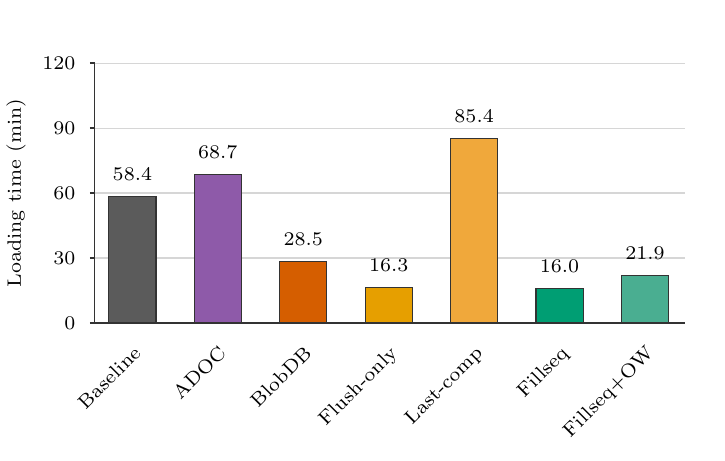
\begin{tikzpicture}[x=1cm,y=1cm,font=\small,
axis/.style={draw=black!80,line width=0.5pt},
grid/.style={draw=black!16,line width=0.4pt}]
\path[use as bounding box] (0,0) rectangle (8.500,5.150);
\draw[grid] (0.85,1.4000) -- (8.3500,1.4000);
\draw[axis] (0.79,1.4000) -- (0.85,1.4000);
\node[font=\fontsize{7}{8}\selectfont,anchor=east] at (0.7300,1.4000) {0};
\draw[grid] (0.85,2.2250) -- (8.3500,2.2250);
\draw[axis] (0.79,2.2250) -- (0.85,2.2250);
\node[font=\fontsize{7}{8}\selectfont,anchor=east] at (0.7300,2.2250) {30};
\draw[grid] (0.85,3.0500) -- (8.3500,3.0500);
\draw[axis] (0.79,3.0500) -- (0.85,3.0500);
\node[font=\fontsize{7}{8}\selectfont,anchor=east] at (0.7300,3.0500) {60};
\draw[grid] (0.85,3.8750) -- (8.3500,3.8750);
\draw[axis] (0.79,3.8750) -- (0.85,3.8750);
\node[font=\fontsize{7}{8}\selectfont,anchor=east] at (0.7300,3.8750) {90};
\draw[grid] (0.85,4.7000) -- (8.3500,4.7000);
\draw[axis] (0.79,4.7000) -- (0.85,4.7000);
\node[font=\fontsize{7}{8}\selectfont,anchor=east] at (0.7300,4.7000) {120};
\draw[axis] (0.85,1.4000) -- (8.3500,1.4000);
\draw[axis] (0.85,1.4000) -- (0.85,4.7000);
\node[font=\fontsize{7}{8}\selectfont,rotate=90,anchor=south] at (0.1000,3.0500) {Loading time (min)};
% baseline: 58.35695416 min
\draw[draw=black!80,line width=0.4pt,fill=vb0] (1.03000,1.40000) rectangle (1.63000,3.00482);
\node[font=\fontsize{7}{8}\selectfont,anchor=south] at (1.3300,3.0848) {58.4};
\node[font=\fontsize{7}{8}\selectfont,rotate=45,anchor=north east] at (1.3300,1.3000) {Baseline};
% adoc: 68.70000000 min
\draw[draw=black!80,line width=0.4pt,fill=vb1] (2.11500,1.40000) rectangle (2.71500,3.28925);
\node[font=\fontsize{7}{8}\selectfont,anchor=south] at (2.4150,3.3693) {68.7};
\node[font=\fontsize{7}{8}\selectfont,rotate=45,anchor=north east] at (2.4150,1.3000) {ADOC};
% blobdb: 28.53330000 min
\draw[draw=black!80,line width=0.4pt,fill=vb2] (3.20000,1.40000) rectangle (3.80000,2.18467);
\node[font=\fontsize{7}{8}\selectfont,anchor=south] at (3.5000,2.2647) {28.5};
\node[font=\fontsize{7}{8}\selectfont,rotate=45,anchor=north east] at (3.5000,1.3000) {BlobDB};
% flush_only: 16.32876947 min
\draw[draw=black!80,line width=0.4pt,fill=vb3] (4.28500,1.40000) rectangle (4.88500,1.84904);
\node[font=\fontsize{7}{8}\selectfont,anchor=south] at (4.5850,1.9290) {16.3};
\node[font=\fontsize{7}{8}\selectfont,rotate=45,anchor=north east] at (4.5850,1.3000) {Flush-only};
% last_comp: 85.37579887 min
\draw[draw=black!80,line width=0.4pt,fill=vb4] (5.37000,1.40000) rectangle (5.97000,3.74783);
\node[font=\fontsize{7}{8}\selectfont,anchor=south] at (5.6700,3.8278) {85.4};
\node[font=\fontsize{7}{8}\selectfont,rotate=45,anchor=north east] at (5.6700,1.3000) {Last-comp};
% fillseq: 16.04406701 min
\draw[draw=black!80,line width=0.4pt,fill=vb5] (6.45500,1.40000) rectangle (7.05500,1.84121);
\node[font=\fontsize{7}{8}\selectfont,anchor=south] at (6.7550,1.9212) {16.0};
\node[font=\fontsize{7}{8}\selectfont,rotate=45,anchor=north east] at (6.7550,1.3000) {Fillseq};
% fillseq_ow: 21.91005647 min
\draw[draw=black!80,line width=0.4pt,fill=vb6] (7.54000,1.40000) rectangle (8.14000,2.00253);
\node[font=\fontsize{7}{8}\selectfont,anchor=south] at (7.8400,2.0825) {21.9};
\node[font=\fontsize{7}{8}\selectfont,rotate=45,anchor=north east] at (7.8400,1.3000) {Fillseq+OW};
\end{tikzpicture}
\endgroup
